\chapter{Judges 17}

\begin{figure}
  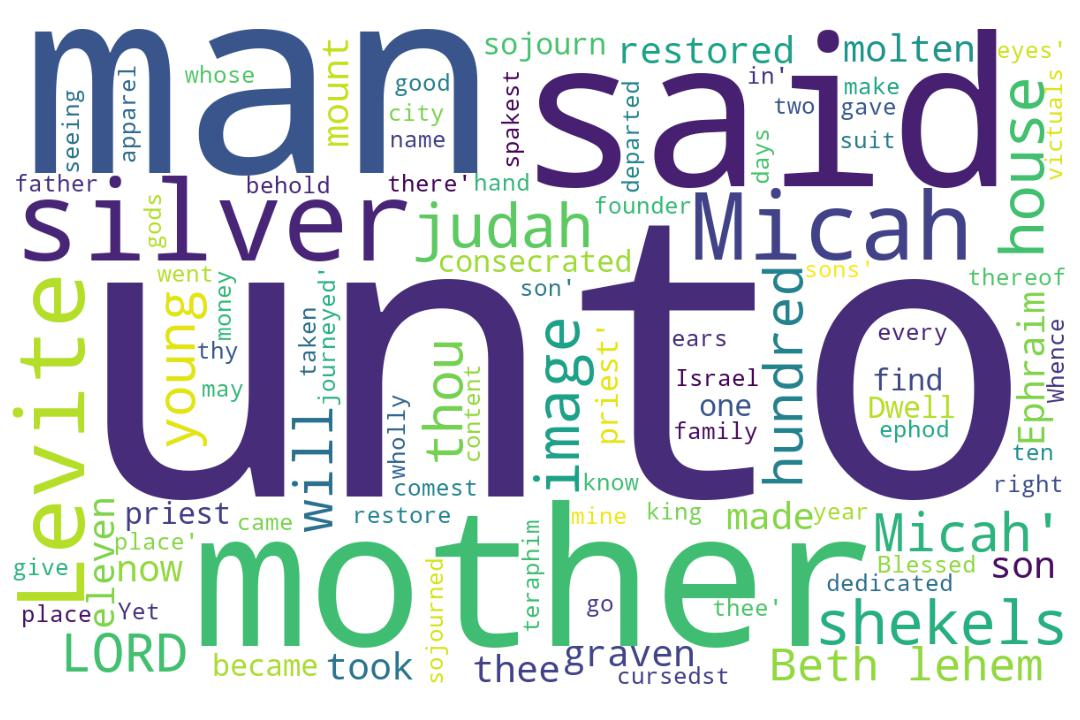
\includegraphics[width=\linewidth]{07OT-Judges/Judges17-WordCloud.jpg}
  \caption{Judges 17 Word Cloud}
  \label{fig:Judges 17 Word Cloud}
\end{figure}

\marginpar{\scriptsize \centering \fcolorbox{bone}{lime}{BUYING A PRIEST}\\ (Judges 17) \begin{compactenum}[I.][8]
    \item  The \textbf{Silver} \index[scripture]{Judges!Jdg 17:02} (Jdg 17:2) 
    \item  A \textbf{Statue} \index[scripture]{Judges!Jdg 17:04} (Jdg 17:4) 
    \item  A \textbf{Shrine} \index[scripture]{Judges!Jdg 17:05} (Jdg 17:5) 
    \item  The \textbf{Selection} \index[scripture]{Judges!Jdg 17:05} (Jdg 17:5) 
    \item  The \textbf{Sojourning} \index[scripture]{Judges!Jdg 17:07} (Jdg 17:7) 
    \item  The \textbf{Salary} \index[scripture]{Judges!Jdg 17:10} (Jdg 17:10) 
    \item  \textbf{Situational Reasoning} %\index[scripture]{Judges!Judges 17:05} (Jdg 17:5) 
\end{compactenum}}



\footnote{\textcolor[rgb]{0.00,0.25,0.00}{\hyperlink{TOC}{Return to end of Table of Contents.}}}\footnote{\href{https://audiobible.com/bible/judges_17.html}{\textcolor[cmyk]{0.99998,1,0,0}{Judges 17 Audio}}}\textcolor[cmyk]{0.99998,1,0,0}{And there was a man of mount Ephraim, whose name \emph{was} Micah.}
[2] \textcolor[cmyk]{0.99998,1,0,0}{And he said unto his mother, The eleven hundred \emph{shekels} of \fcolorbox{bone}{lime}{silver} that were taken from thee, about which thou cursedst, and spakest of also in mine ears, behold, the silver \emph{is} with me; I took it. And his mother said, Blessed \emph{be} \emph{thou} of the LORD, my son.}
[3] \textcolor[cmyk]{0.99998,1,0,0}{And when he had restored the eleven hundred \emph{shekels} of silver to his mother, his mother said, I had wholly dedicated the silver unto the LORD from my hand for my son, to make a graven image and a molten image: now therefore I will restore it unto thee.}
[4] \textcolor[cmyk]{0.99998,1,0,0}{Yet he restored the money unto his mother; and his mother took two hundred \emph{shekels} of silver, and gave them to the founder, who made thereof a graven image and a molten \fcolorbox{bone}{lime}{image}: and they were in the house of Micah.}
[5] \textcolor[cmyk]{0.99998,1,0,0}{And the man Micah had an \fcolorbox{bone}{lime}{house} of gods, and made an ephod, and teraphim, and consecrated one of his \fcolorbox{bone}{lime}{sons}, who became his priest.}
[6] \textcolor[cmyk]{0.99998,1,0,0}{In those days \emph{there} \emph{was} no king in Israel, \emph{but} every man did \emph{that} \emph{which} \emph{was} right in his own eyes.}\footnote{\textbf{Proverb 14:12} - There is a way which seemeth right unto a man, but the end thereof \emph{are} the ways of death.}\\
\\
\P\textcolor[cmyk]{0.99998,1,0,0}{And there was a young man out of Beth-lehem-judah of the family of Judah, who \emph{was} a Levite, and he \fcolorbox{bone}{lime}{sojourned} there.}
[8] \textcolor[cmyk]{0.99998,1,0,0}{And the man departed out of the city from Beth-lehem-judah to sojourn where he could find \emph{a} \emph{place}: and he came to mount Ephraim to the house of Micah, as he journeyed.}
[9] \textcolor[cmyk]{0.99998,1,0,0}{And Micah said unto him, Whence comest thou? And he said unto him, I \emph{am} a Levite of Beth-lehem-judah, and I go to sojourn where I may find \emph{a} \emph{place}.}
[10] \textcolor[cmyk]{0.99998,1,0,0}{And Micah said unto him, Dwell with me, and be unto me a father and a priest, and I will give thee ten \fcolorbox{bone}{lime}{\emph{shekels}} of silver by the year, and a suit of apparel, and thy victuals. So the Levite went in.}
[11] \textcolor[cmyk]{0.99998,1,0,0}{And the Levite was content to dwell with the man; and the young man was unto him as one of his sons.}
[12] \textcolor[cmyk]{0.99998,1,0,0}{And Micah consecrated the Levite; and the young man became his priest, and was in the house of Micah.}
[13] \textcolor[cmyk]{0.99998,1,0,0}{Then said Micah, Now know I that the LORD will do me good, \fcolorbox{bone}{lime}{\emph{seeing}} I have a Levite to \emph{my} priest.}